\documentclass{article}

\usepackage[utf8]{inputenc}
\usepackage{graphicx}
\usepackage{tikz}
\usepackage{float}
\usepackage{wrapfig,lipsum}
\usepackage{svg}
\usepackage{mathtools}
\usepackage{tabu}
%\usepackage{subcaption}
\usepackage{subfigure}
\usepackage[a4paper, total={6in, 8in}]{geometry}


\begin{document}


\newcommand{\vecthreeBF}[1]{\vec{\textbf{#1}}}
\newcommand{\vecthree}[1]{\vec{#1}}

\newcommand{\parDeriv}[2]{\frac{\partial #1}{\partial #2}}
\newcommand{\parDerivS}[2]{\frac{\partial^2 #1}{\partial #2^2}}
\newcommand{\derivS}[2]{\frac{d^2 #1}{d#2^2}}

\newcommand{\dotProdBF}[2]{\vecthreeBF{#1} \cdot \vecthreeBF{#2}}
\newcommand{\dotProd}[2]{\vecthree{#1} \cdot \vecthree{#2}}

\newcommand{\crossProdBF}[2]{\vecthreeBF{#1} \times \vecthreeBF{#2}}
\newcommand{\crossProd}[2]{\vecthree{#1} \times \vecthree{#2}}


\newcommand{\fromeq}[1]{\textit{equation \ref{eq:#1}}}
\newcommand{\fromeqs}[2]{\textit{equations \ref{eq:#1} and \ref{eq:#2}}}
\newcommand{\fromeqsth}[3]{\textit{equations \ref{eq:#1}, \ref{eq:#2} and \ref{eq:#3}}}

\newcommand{\fromfig}[1]{\textit{figure \ref{fig:#1}}}
\newcommand{\fromfigs}[2]{\textit{figures \ref{fig:#1} and \ref{fig:#2}}}

\newcommand{\fromsec}[1]{\textit{section \ref{sec:#1}}}
\newcommand{\fromsecs}[2]{\textit{sections \ref{sec:#1} and \ref{sec:#2}}}

%----../../..++++.

%%%%%%

\section{Initial Design at KAHVELab} 

A rhodotron with operation frequency of $107.5$ MHz was decided to be built at KAHVELab. 
Frequency was selected to benefit from the RF power supply units at hand.
After considering the earlier simulations mentioned in \fromsecs{cavity_design}{magnet_design}, an initial design was created.
\begin{figure}[H]
    \centering
    %%\captionsetup{justification=centering}
    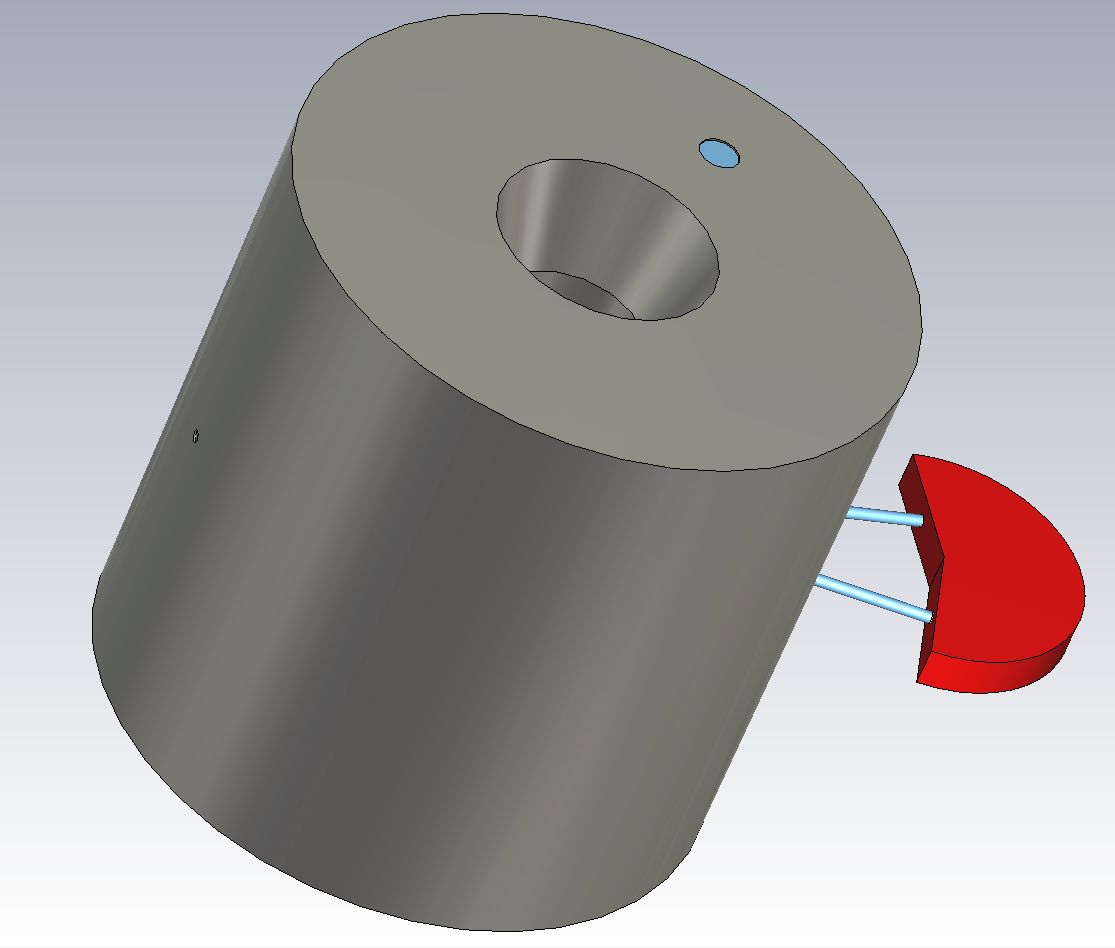
\includegraphics[width=.5\linewidth]{../../../figures/cst/cst_first_design1.png}
    \caption{Initial design of the proposed rhodotron, $\gamma=9^\circ$.}
    \label{fig:initial_design}
\end{figure}
\iffalse \begin{figure}[H]
    %\captionsetup[subfigure]{justification=centering}
    %\captionsetup{justification=centering}
    \centering
    \begin{subfigure}{.5\textwidth}
      \centering
      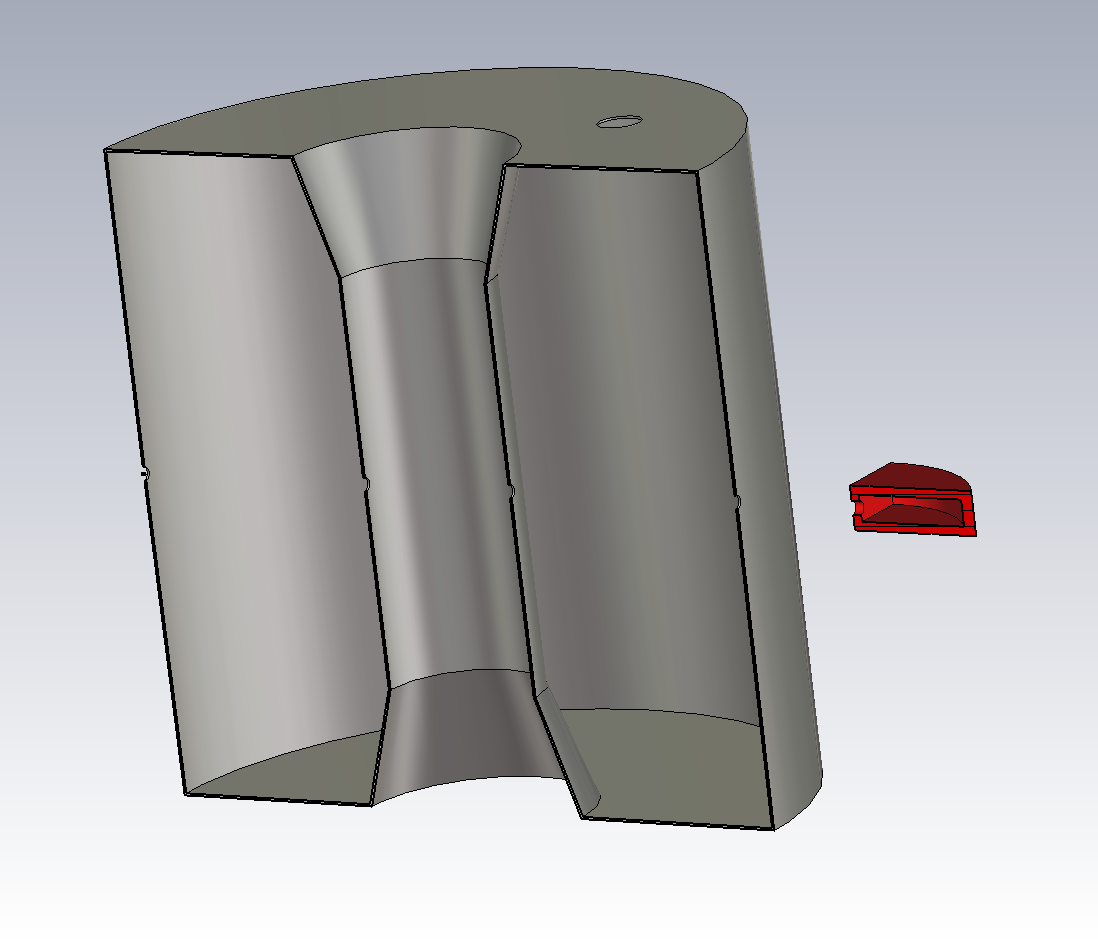
\includegraphics[width=.92\linewidth]{../../../figures/cst/cst_first_design3.png}
      \caption{Axial cross section.}
    \end{subfigure}%
    \centering
    \begin{subfigure}{.5\textwidth}
      \centering
      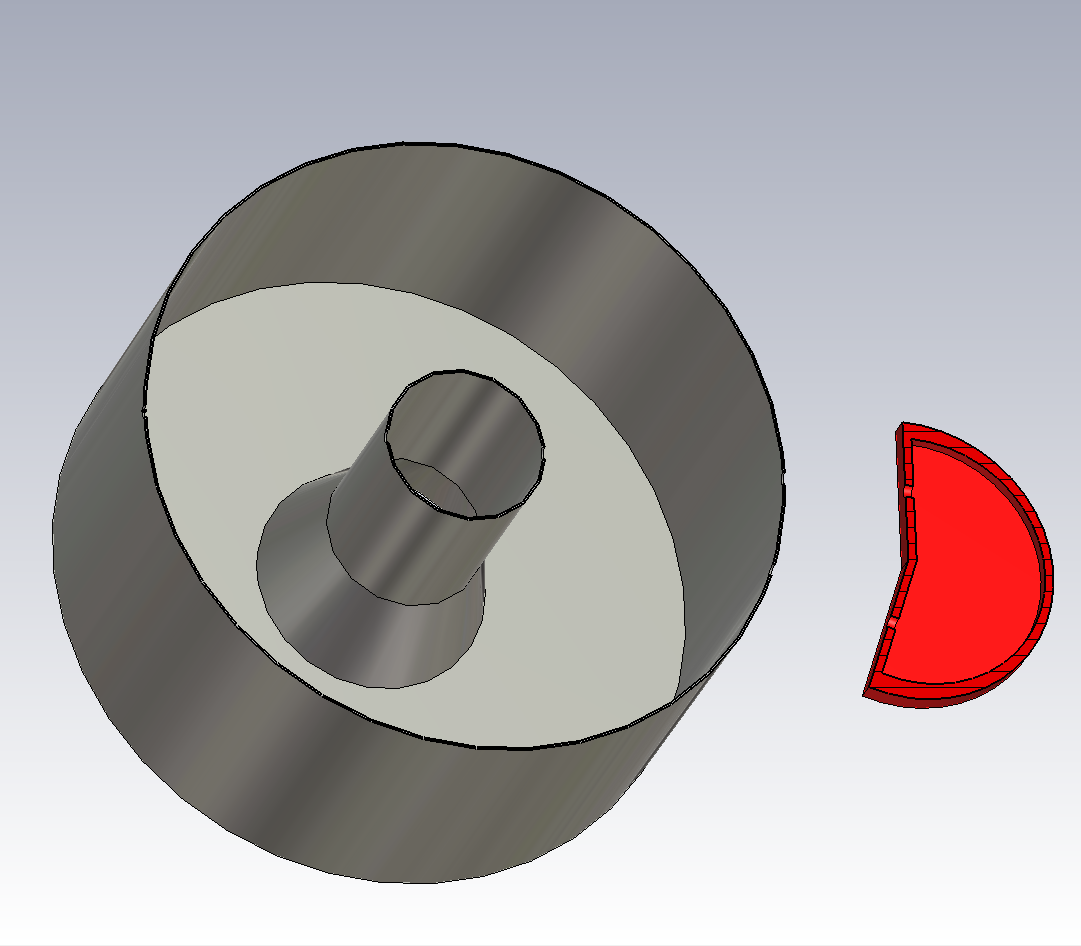
\includegraphics[width=.9\linewidth]{../../../figures/cst/cst_first_design2.png}
      \caption{Cross section at acceleration plane.}
    \end{subfigure}
    \caption{Initial design of the proposed rhodotron.}
    \label{fig:initial_design_cross_section}
\end{figure} \fi
\begin{figure}[H]
    \centering
    \subfigure[\centering Axial cross section]{{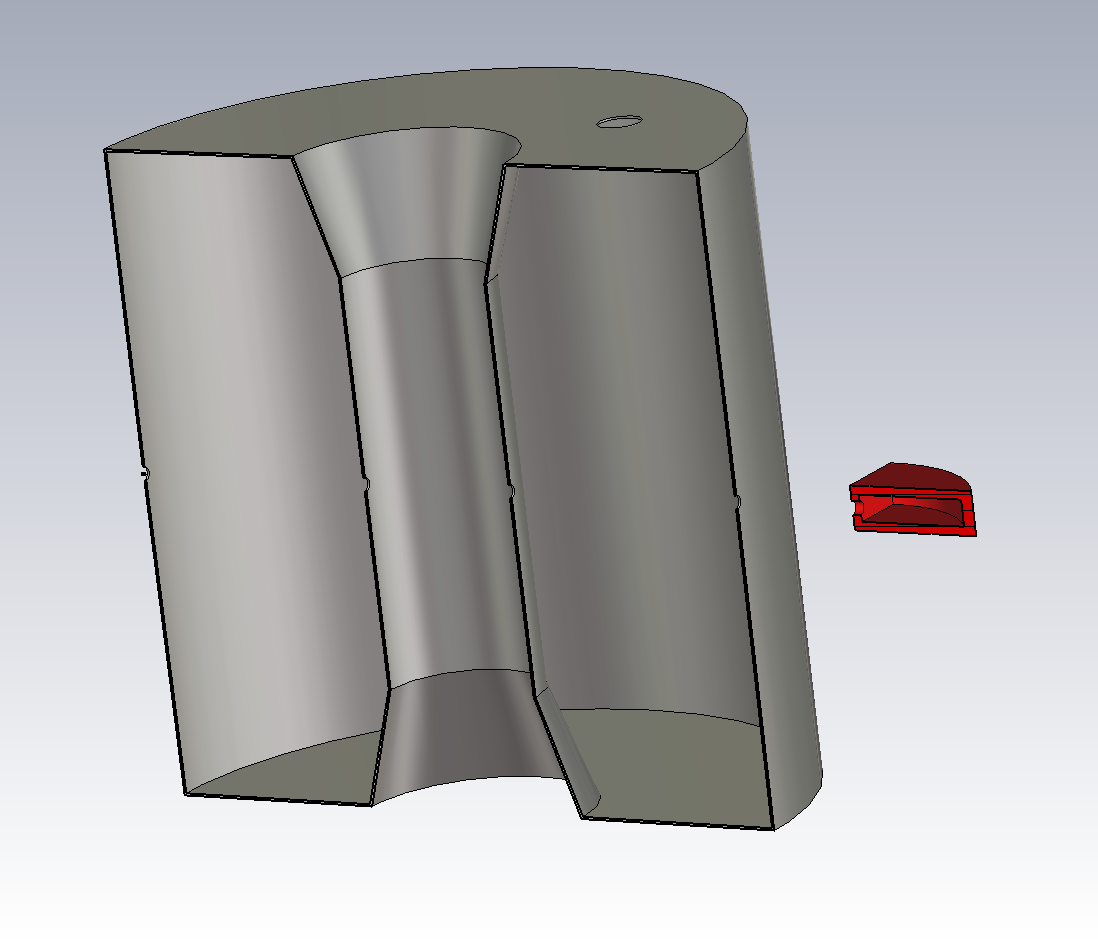
\includegraphics[width=.46\textwidth]{../../../figures/cst/cst_first_design3.png} }}%
    \qquad\subfigure[\centering Cross section at acceleration plane]{{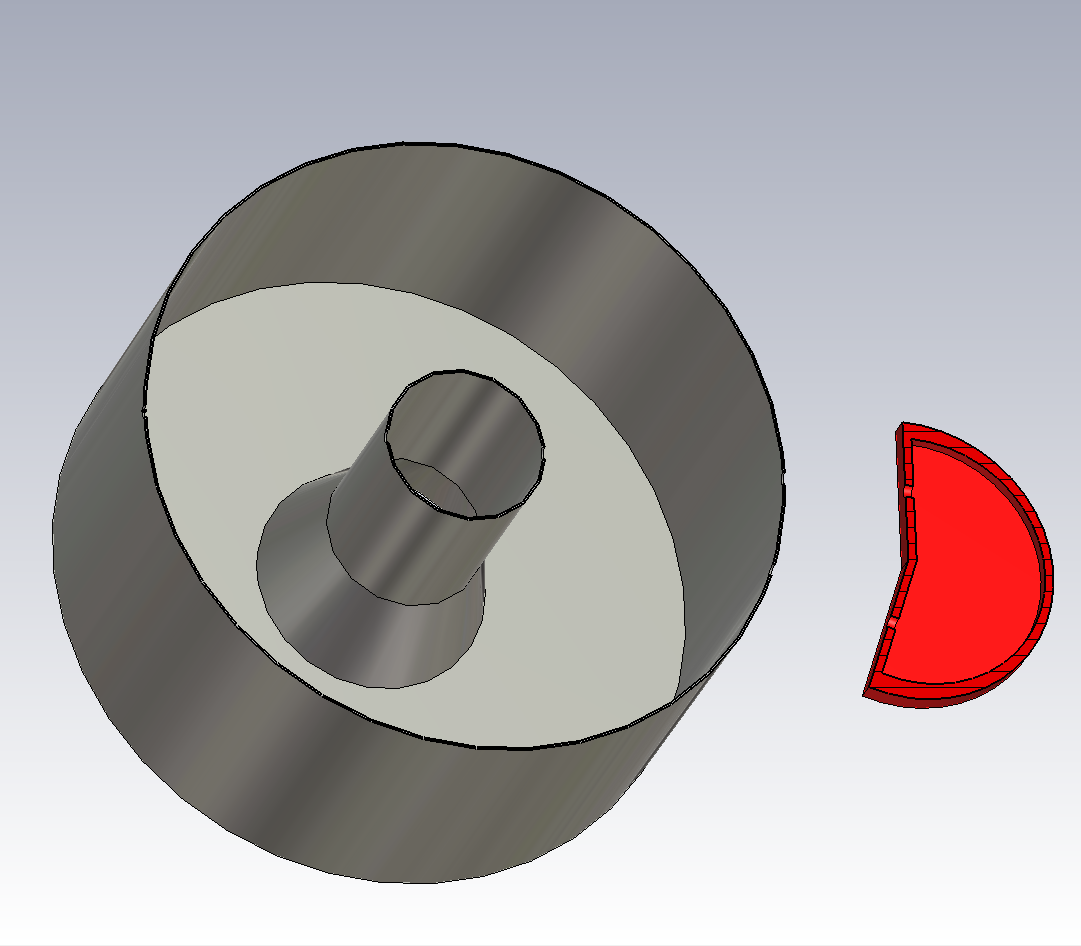
\includegraphics[width=.45\textwidth]{../../../figures/cst/cst_first_design2.png} }}%
    \vspace{20pt}
    \caption{\centering Initial design of the proposed rhodotron.} 
    \label{fig:initial_design_cross_section}
\end{figure}
The magnets used in this design is the simplest in terms of design parameters. It consists of an iron casing encapsulating the shape of desired magnetic field, which are created by two coils inside.
\iffalse \begin{figure}[H]
    %\captionsetup[subfigure]{justification=centering}
    %\captionsetup{justification=centering}
    \centering
    \begin{subfigure}{.5\textwidth}
      \centering
      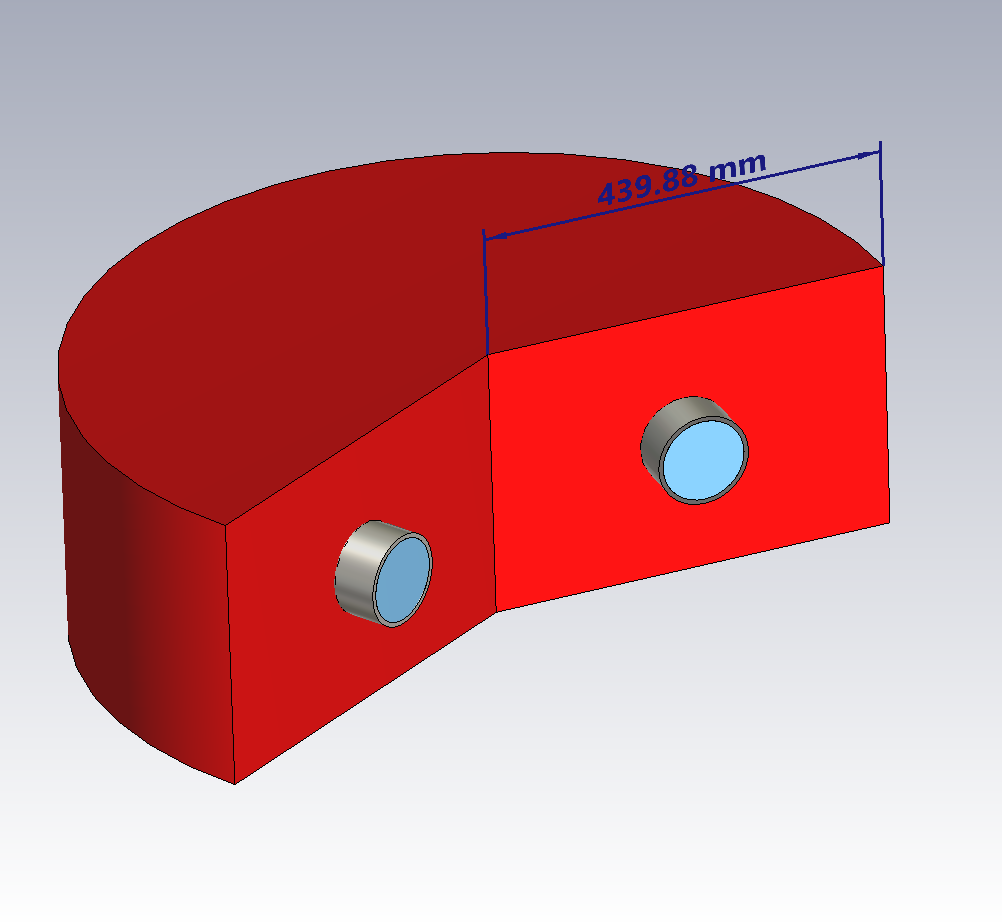
\includegraphics[width=.9\linewidth]{../../../figures/cst/cst_first_magnet_design1.png}
    \end{subfigure}%
    \centering
    \begin{subfigure}{.5\textwidth}
      \centering
      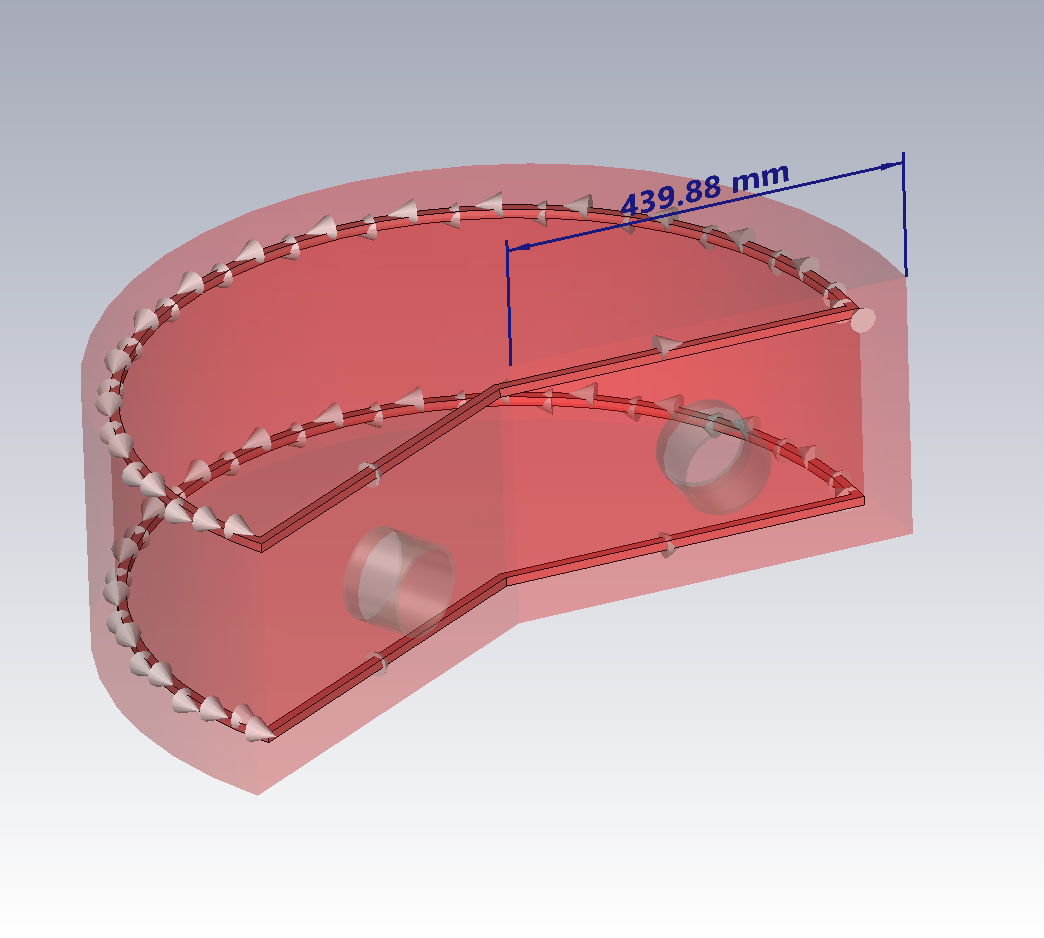
\includegraphics[width=.92\linewidth]{../../../figures/cst/cst_first_magnet_design2.png}
    \end{subfigure}
    \caption{Initial magnet design.}
    \label{fig:initial_magnet_design}
\end{figure} \fi
\begin{figure}[H]
    \centering
    \subfigure[\centering ]{{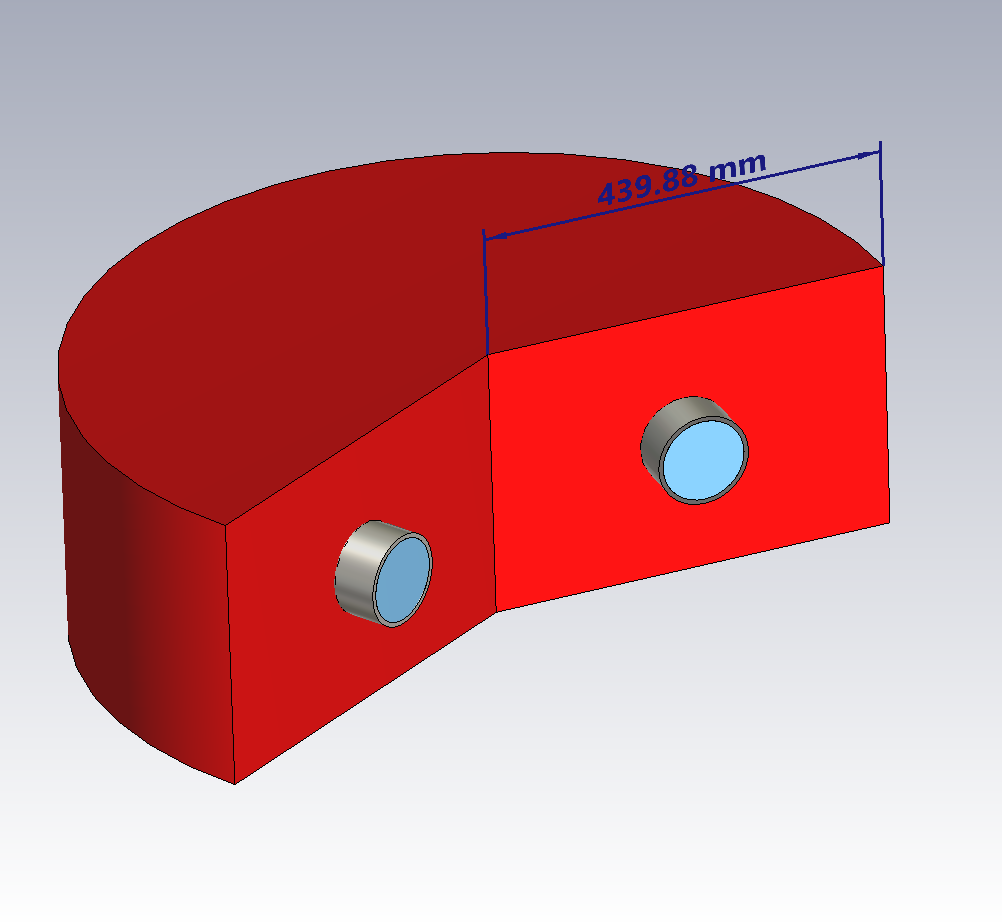
\includegraphics[width=.45\textwidth]{../../../figures/cst/cst_first_magnet_design1.png} }}%
    \qquad\subfigure[\centering ]{{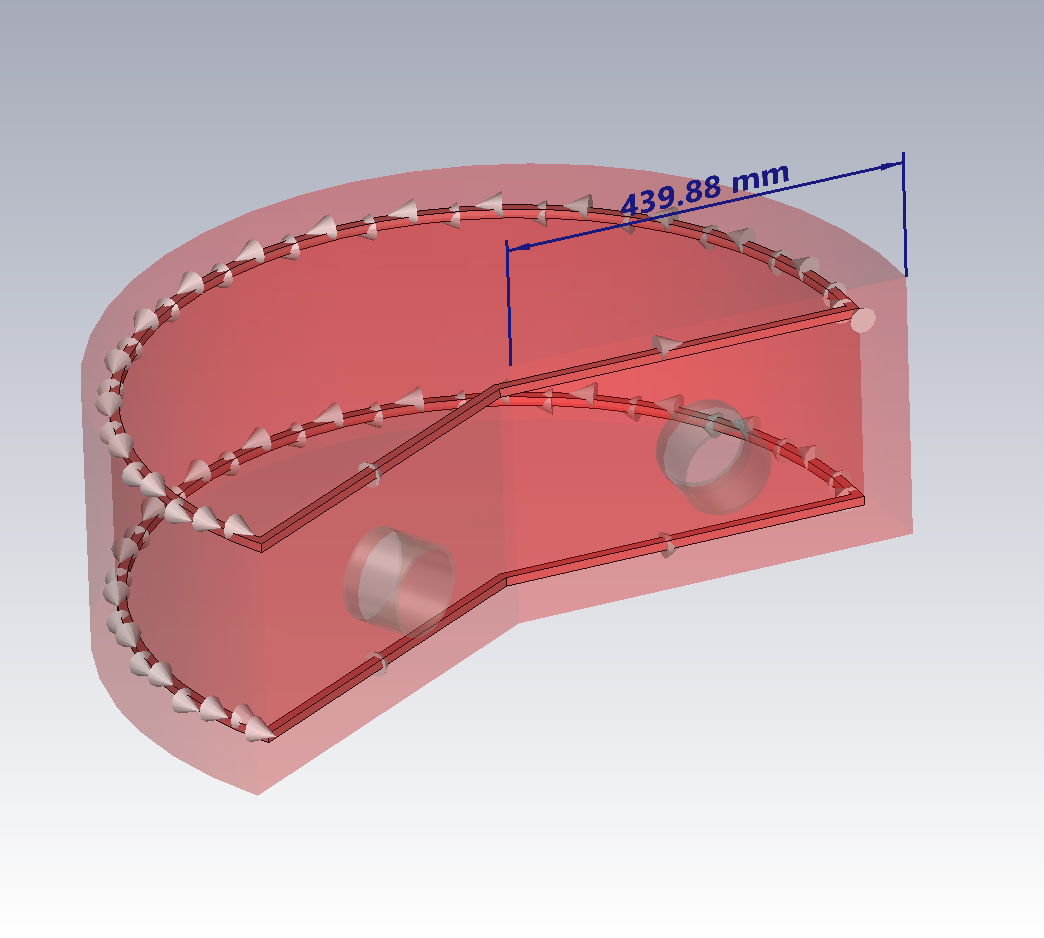
\includegraphics[width=.46\textwidth]{../../../figures/cst/cst_first_magnet_design2.png} }}%
    \vspace{20pt}
    \caption{\centering Initial magnet design.} 
    \label{fig:initial_magnet_design}
\end{figure}

\begin{figure}[H]
    \centering
    %%\captionsetup{justification=centering}
    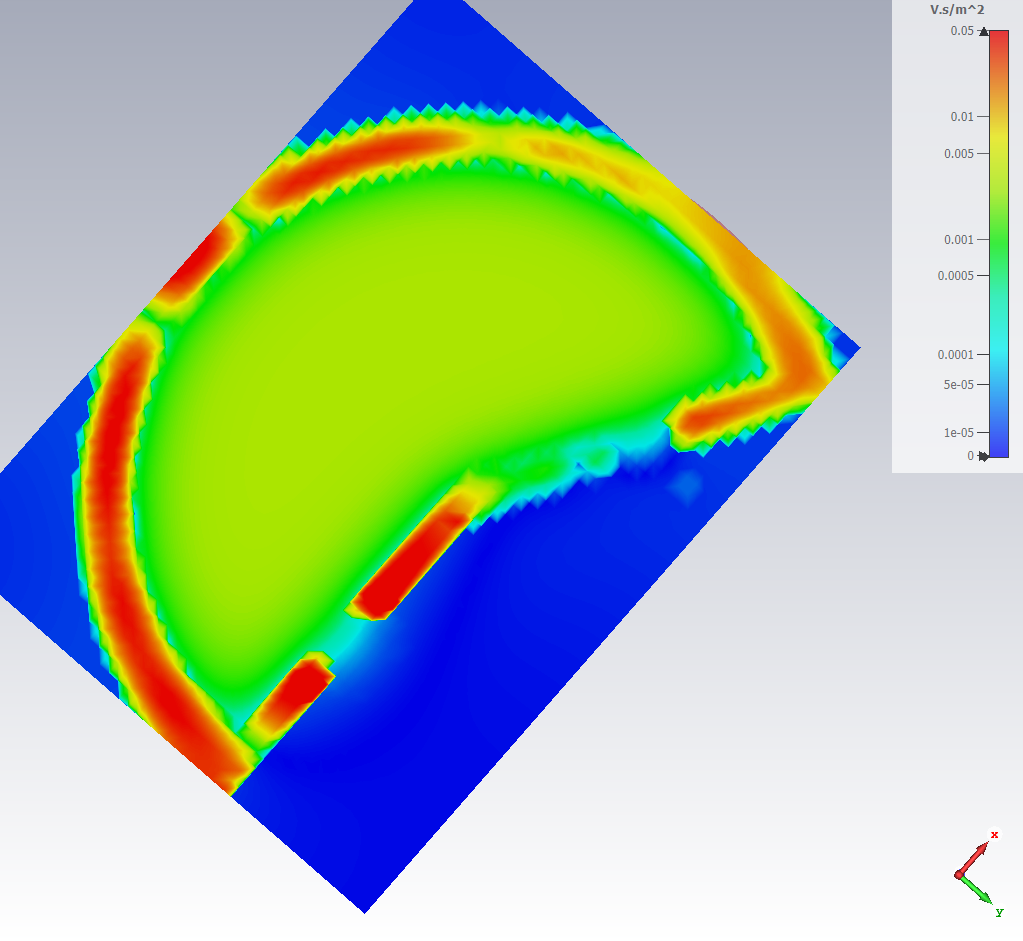
\includegraphics[width=.8\linewidth]{../../../figures/cst/cst_first_magnet_design3.png}
    \caption{Magnetic field in acceleration plate of initial magnet design.}
    \label{fig:initial_magnet_design_B}
\end{figure}
\fromfig{initial_magnet_design_B} shows that this design provides relatively uniform magnetic field inside, although magnetic field gradient in the openings can be improved. 

After adding two more magnets and using $\gamma=15^\circ$, the following second prototype design was created
\begin{figure}[H]
    \centering
    %%\captionsetup{justification=centering}
    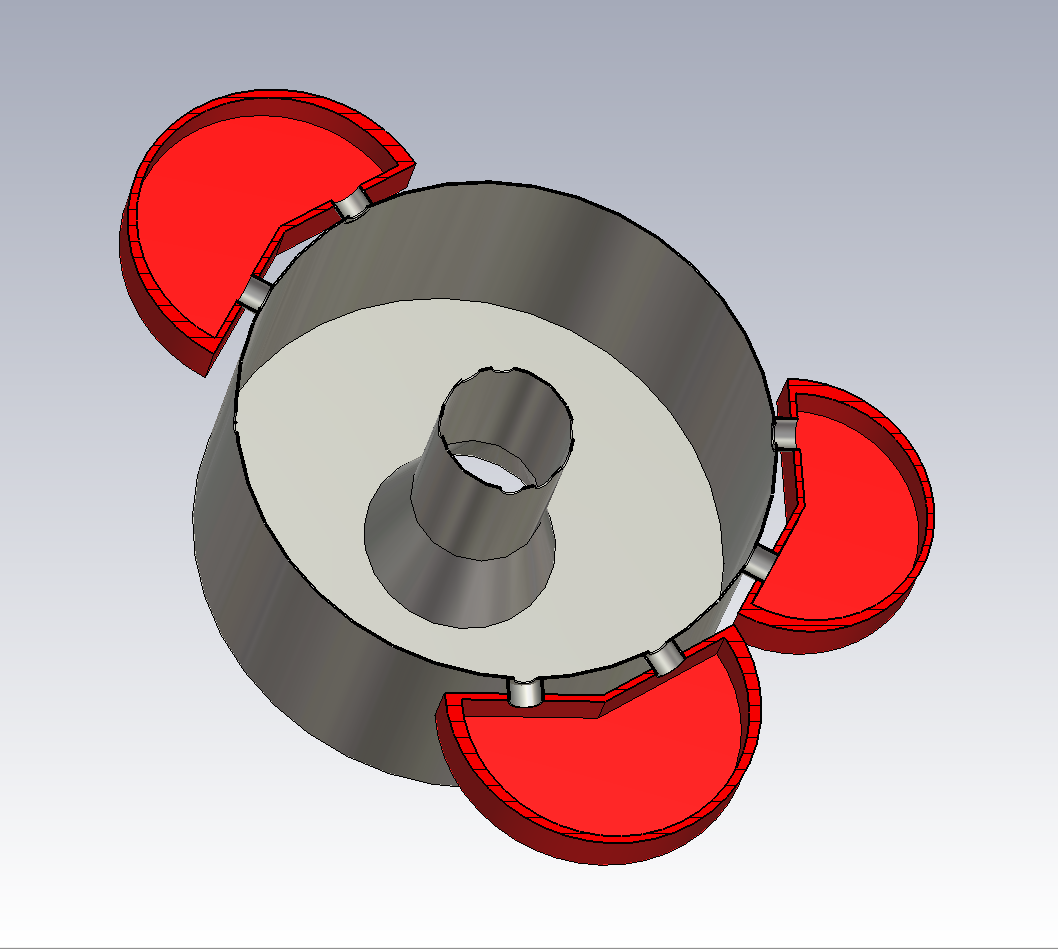
\includegraphics[width=.8\linewidth]{../../../figures/cst/cst_second_design2.png}
    \caption{Initial cavity with three magnets as shown in \fromfig{initial_magnet_design}, $\gamma=15^\circ$.}
    \label{fig:initial_three_magnet_design}
\end{figure}
These designs, together with $40$ keV $e^-$ gun injecting with phase lag of $15^\circ$ for $1$ ns, was simulated at RF power of $12$ kW using \textit{CST Studio Particle Module PIC Solver}.
Results of these simulations can be found in \fromfig{initial_designs_PIC_phase_space_monitor}.
\iffalse \begin{figure}[H]
    %\captionsetup[subfigure]{justification=centering}
    %\captionsetup{justification=centering}
    \centering
    \begin{subfigure}[b]{.8\textwidth}
      \centering
      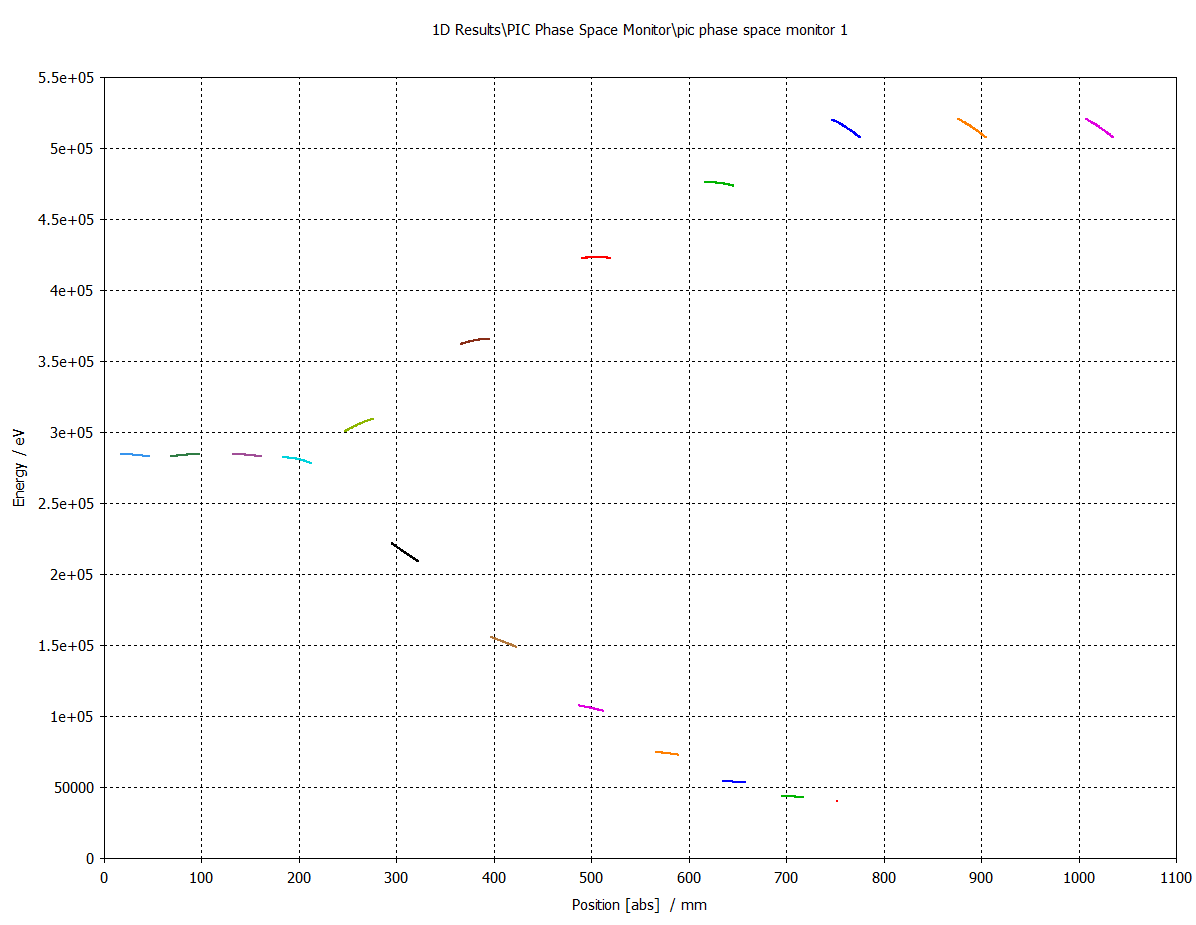
\includegraphics[width=\linewidth]{../../../figures/cst/cst_first_design4.png}
      \caption{One pass simulation of \fromfig{initial_design}}
    \end{subfigure}
    \centering
    \begin{subfigure}[b]{.8\textwidth}
      \centering
      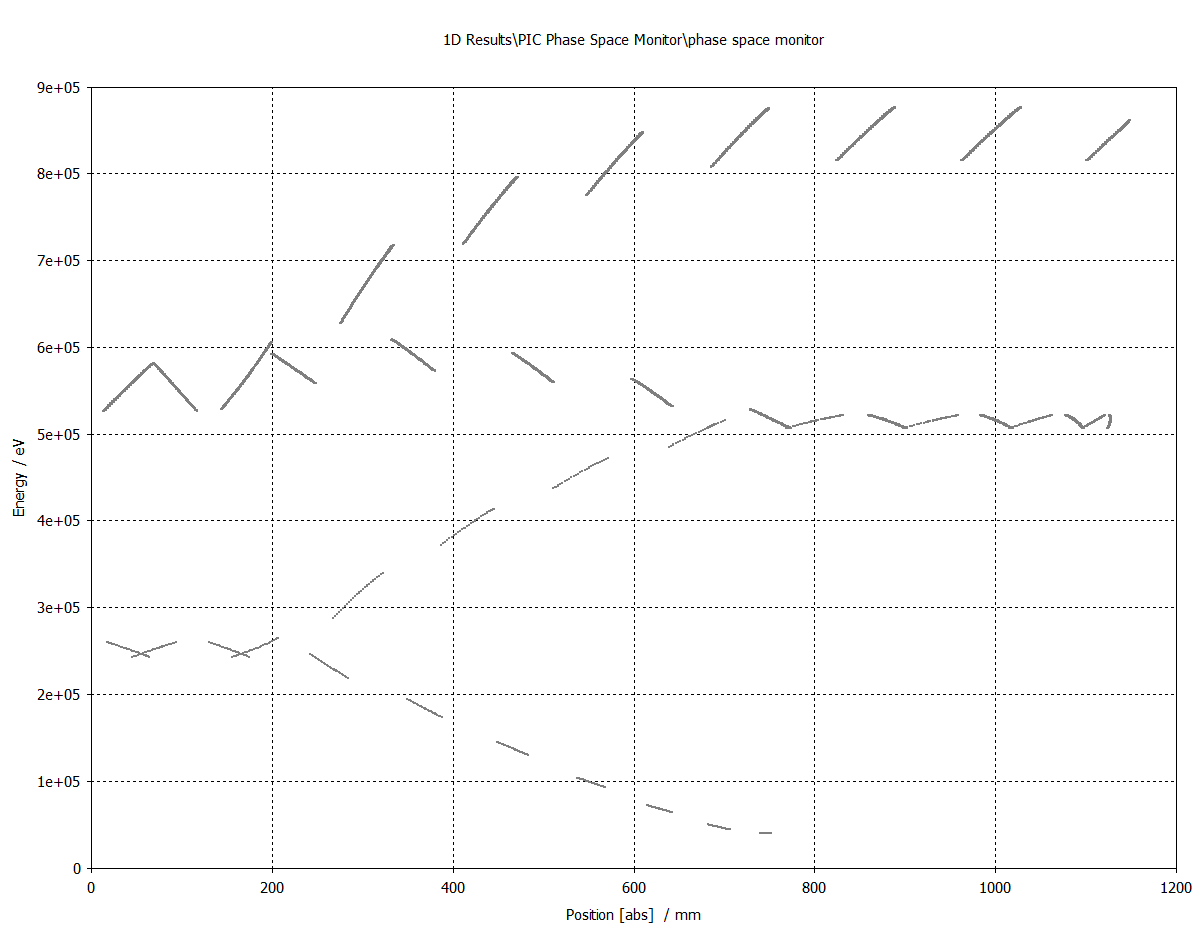
\includegraphics[width=\linewidth]{../../../figures/cst/cst_second_design3.png}
      \caption{Two pass simulation of \fromfig{initial_three_magnet_design}}
    \end{subfigure}
    \caption{$|r|$ vs $Energy$ simulation of initial design.}
    \label{fig:initial_designs_PIC_phase_space_monitor}
\end{figure} \fi
\begin{figure}[H]
    \centering
    \subfigure[\centering One pass simulation of \fromfig{initial_design}]{{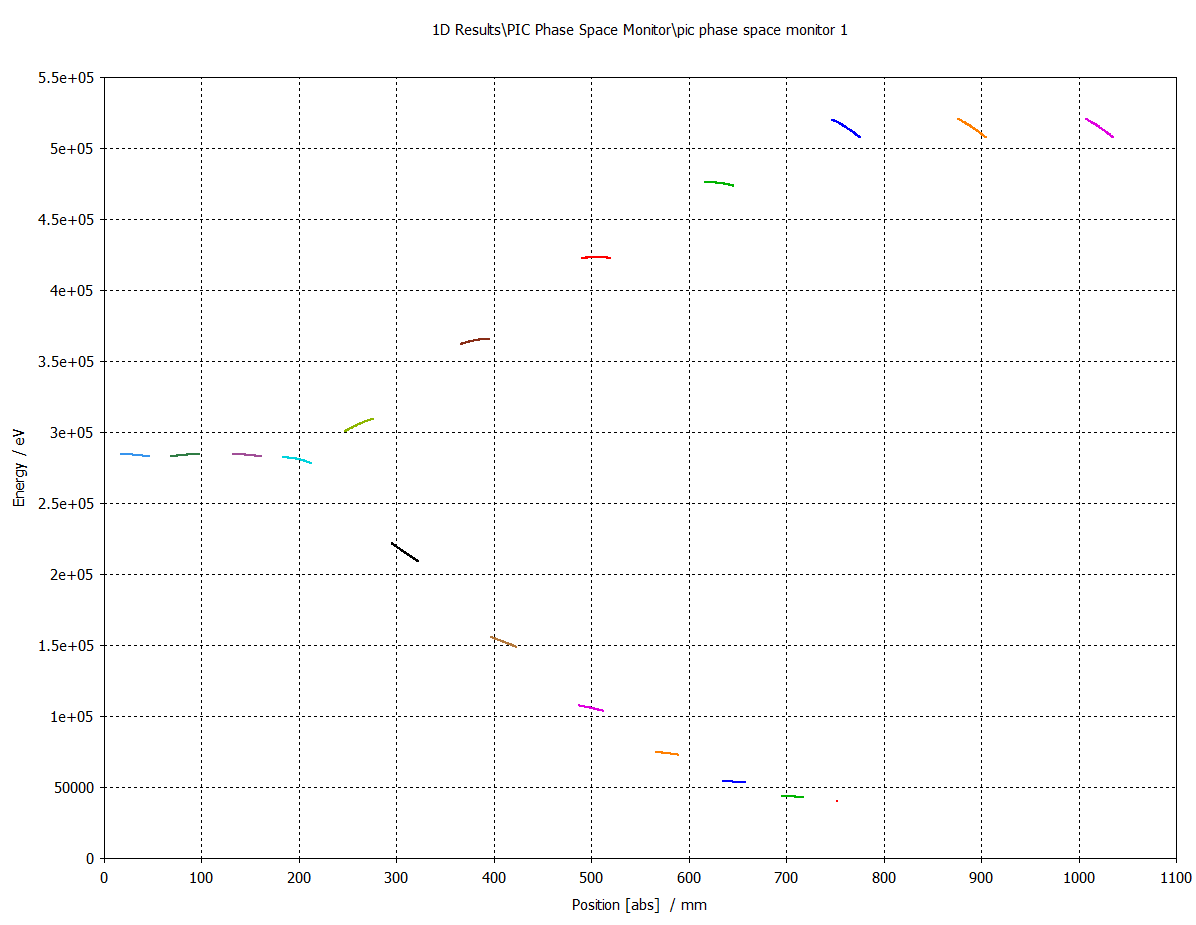
\includegraphics[width=.8\textwidth]{../../../figures/cst/cst_first_design4.png} }}%
    \vspace{20pt}\newline
    \subfigure[\centering Two pass simulation of \fromfig{initial_three_magnet_design}]{{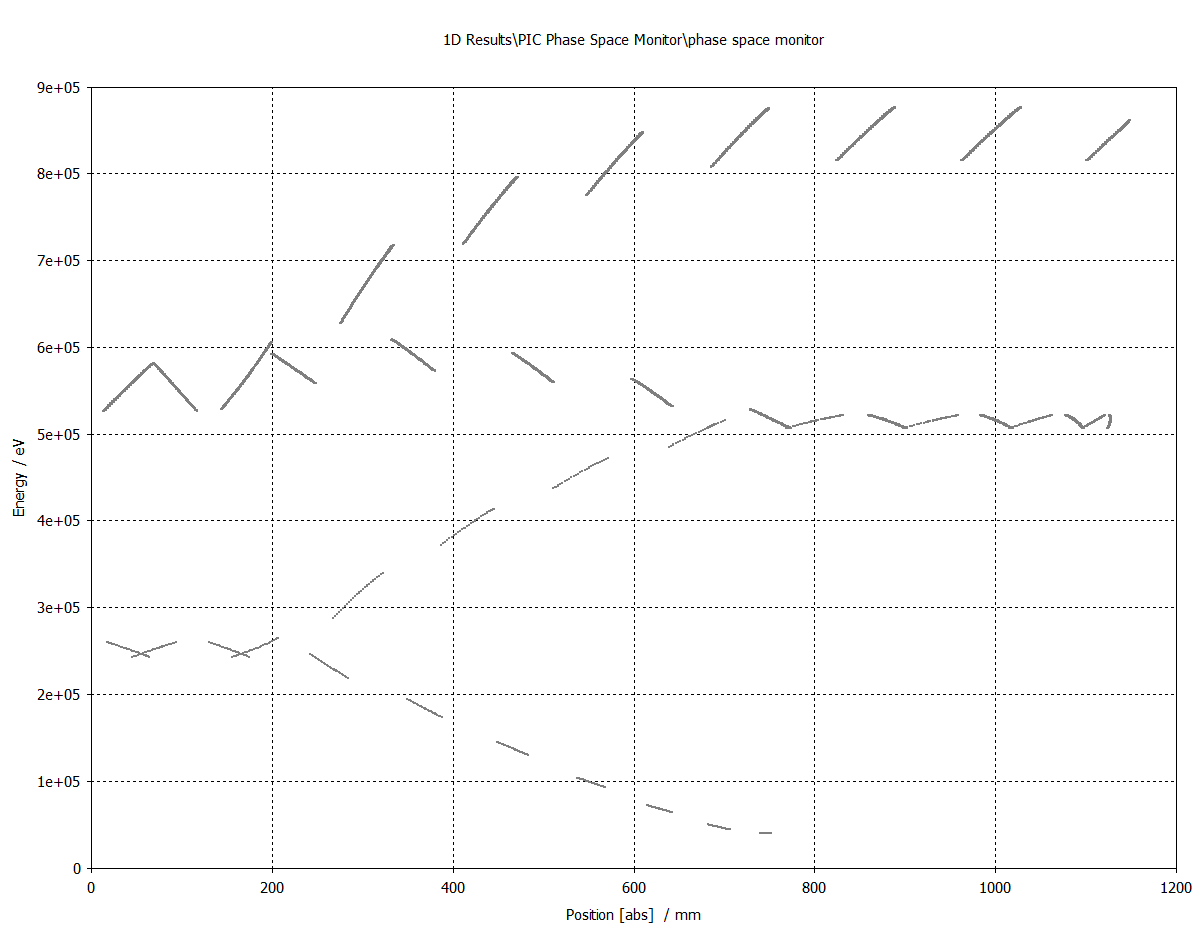
\includegraphics[width=.8\textwidth]{../../../figures/cst/cst_second_design3.png} }}%
    \vspace{20pt}
    \caption{\centering $|r|$ vs $Energy$ simulation of initial design.} 
    \label{fig:initial_designs_PIC_phase_space_monitor}
\end{figure}
The behavior of the beam in the \fromfig{initial_designs_PIC_phase_space_monitor} after the first pass indicates that phase stability is not maintained. 
When the simulation results are examined further, it was observed that the beam started the second pass at $t \approx 12$ ns after the injection. 
Considering the starting phase lag $\phi_{lag}=15^\circ$, this would mean phase lag of the second pass was $\phi_{lag2}=120^\circ$.
This result can be observed in \fromfig{initial_designs_PIC_phase_space_monitor}, as the beam decelerates after a short acceleration in the beginning of the second pass.

After various similar observations in \textit{CST} similations, underlying cause of this problem was thought to be the $L_{pass} = n \lambda$ approach on magnet design failing in low energies, 
as anticipated and discussed earlier in the \fromsec{parameter_sweep}.
\emph{The necessity for an alternative tool, capable of aiding researchers in improving beam behavior, was deemed evident.}

Several improvements were made to KAHVELab Rhodotron initial designs \cite{sinan}. These include curved edges on cavity which reduce the power loss on cavity walls, and redesigned iron casing on magnets for ease of production and maintenance.
Improved designs can be seen in the figures below.
\iffalse \begin{figure}[H]
    %\captionsetup[subfigure]{justification=centering}
    %\captionsetup{justification=centering}
    \centering
    \begin{subfigure}{.5\textwidth}
      \centering
      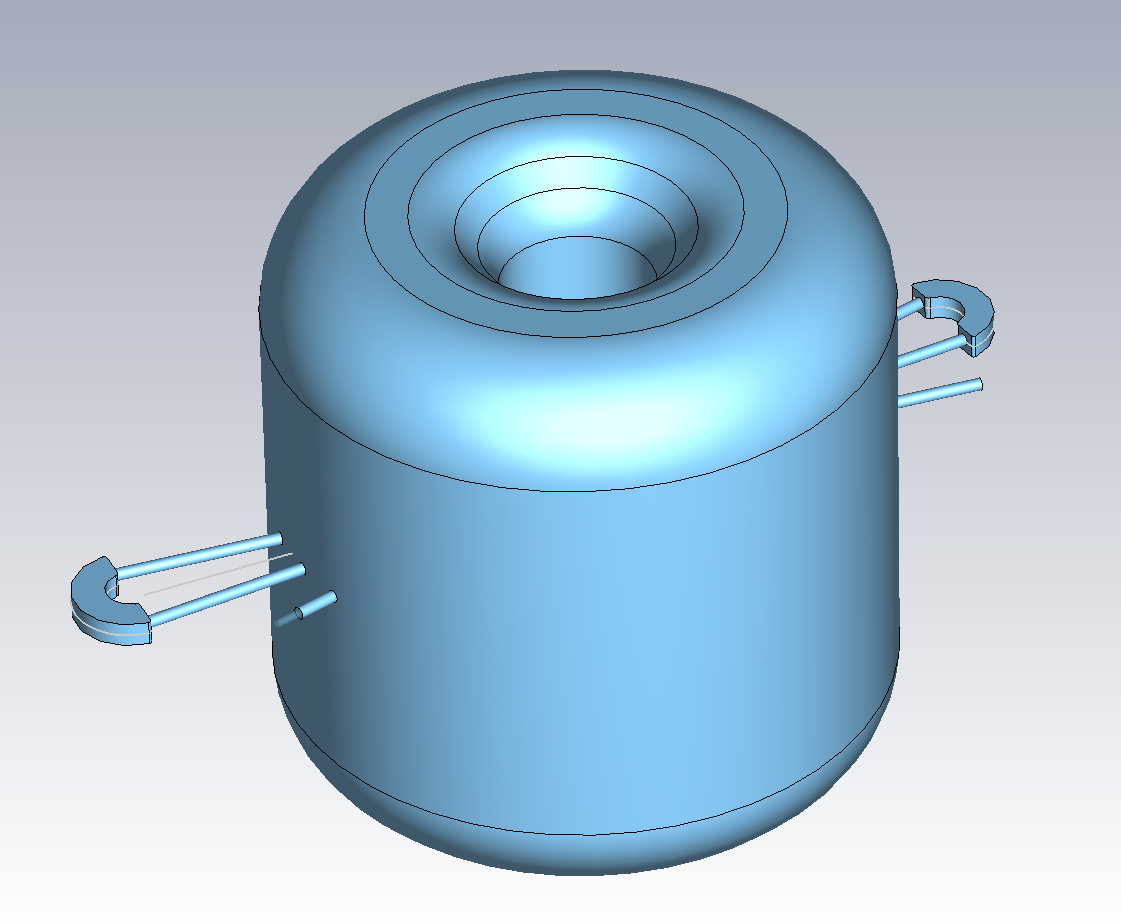
\includegraphics[width=.9\linewidth]{../../../figures/cst/cst_sinan_cavity_design1.png}
    \end{subfigure}%
    \centering
    \begin{subfigure}{.5\textwidth}
      \centering
      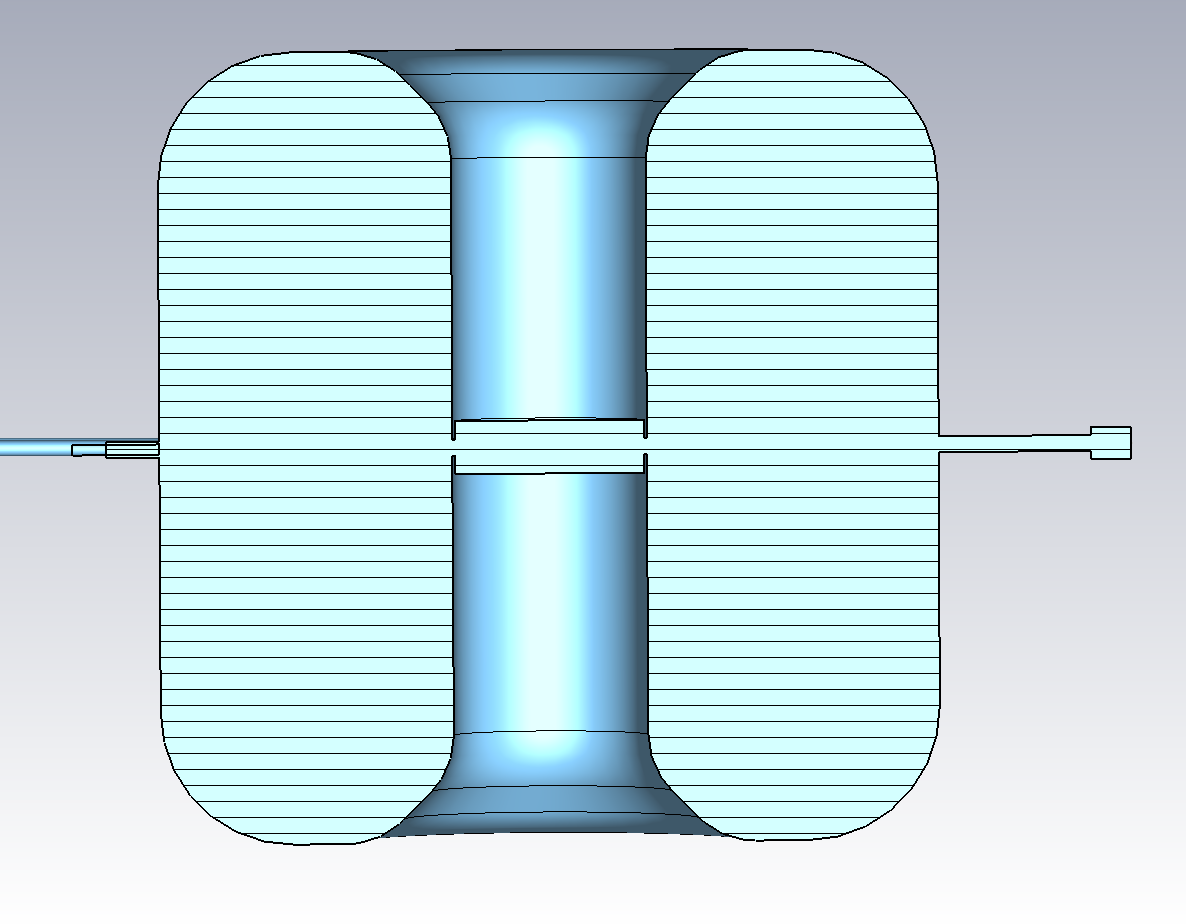
\includegraphics[width=.94\linewidth]{../../../figures/cst/cst_sinan_cavity_design2.png}
    \end{subfigure}
    \caption{Improved cavity design.}
    \label{fig:improved_cavity_design}
\end{figure} \fi
\begin{figure}[H]
    \centering
    \subfigure[\centering ]{{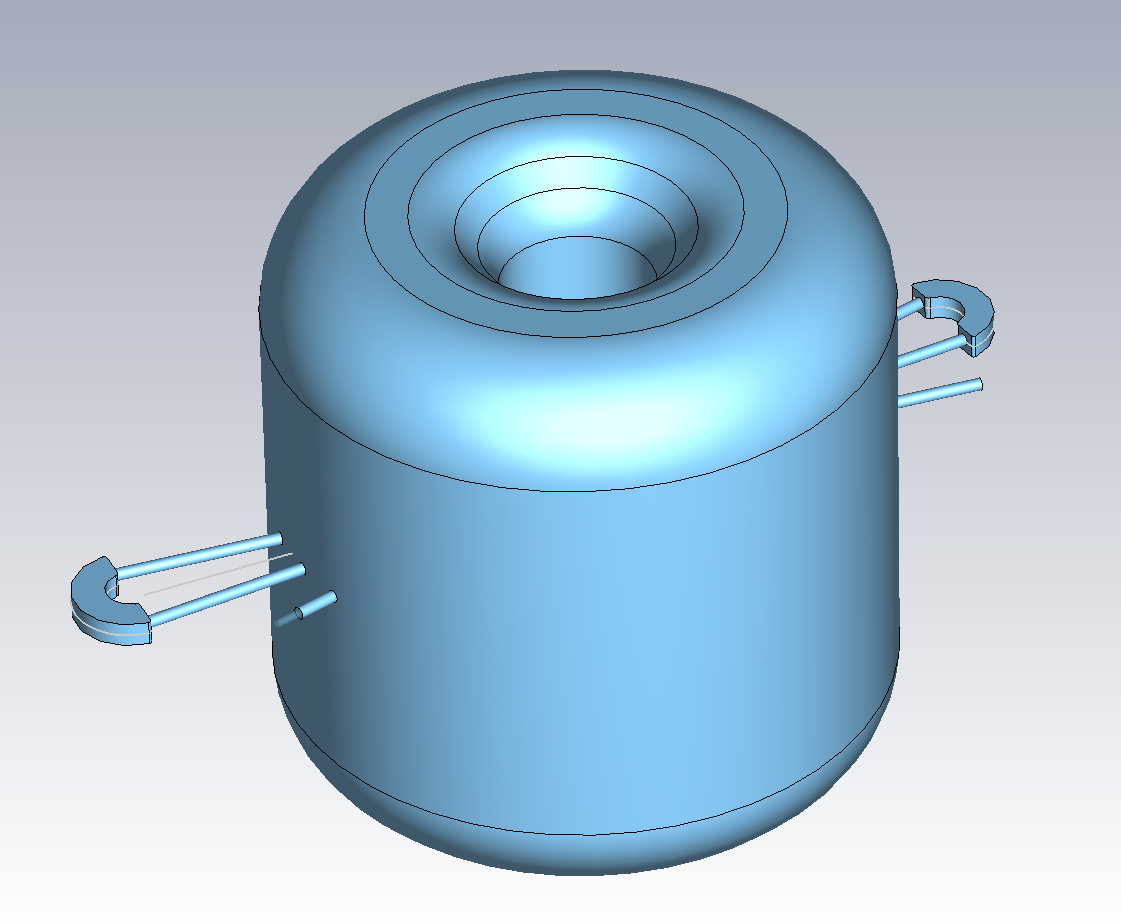
\includegraphics[width=.45\textwidth]{../../../figures/cst/cst_sinan_cavity_design1.png} }}%
    \qquad\subfigure[\centering ]{{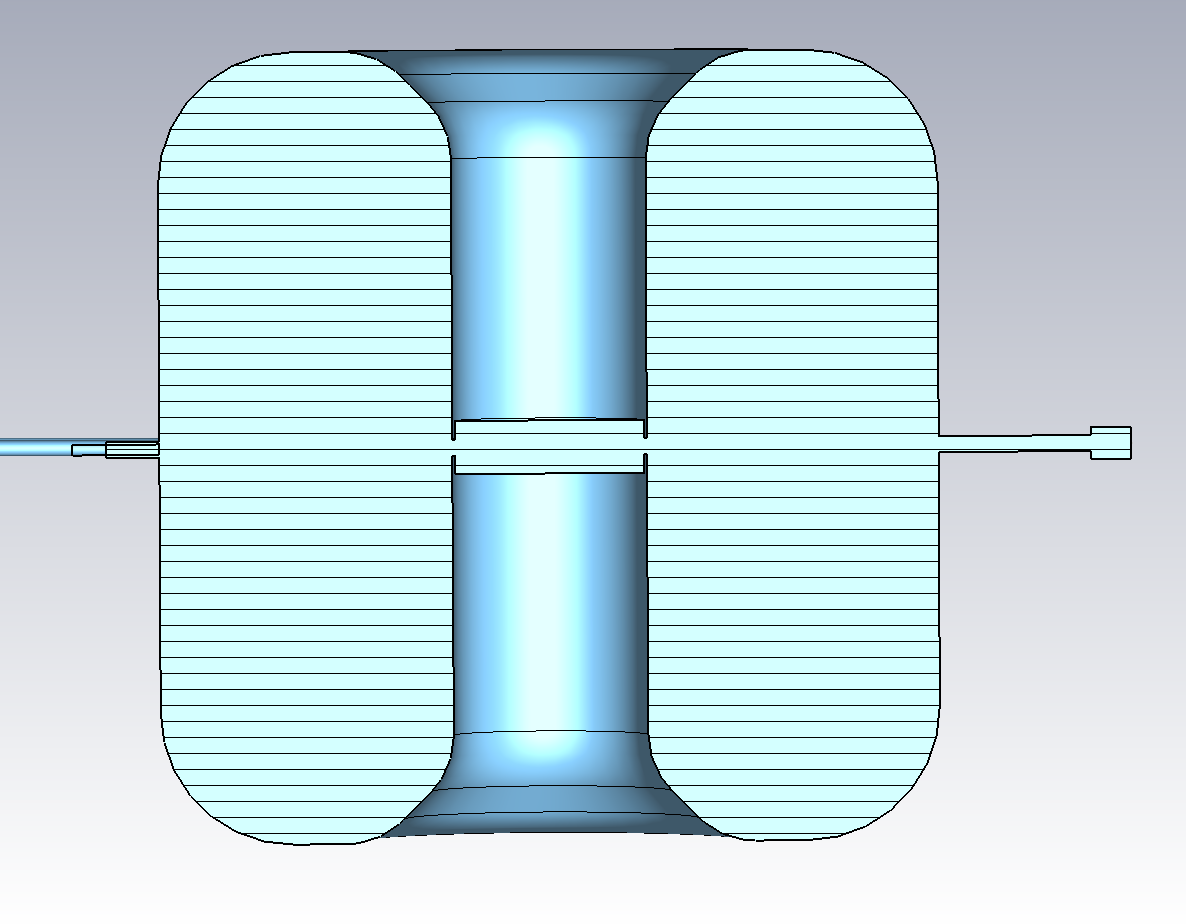
\includegraphics[width=.47\textwidth]{../../../figures/cst/cst_sinan_cavity_design2.png} }}%
    \vspace{20pt}
    \caption{\centering Improved cavity design.} 
    \label{fig:improved_cavity_design}
\end{figure}

\begin{figure}[H]
    \centering
    %%\captionsetup{justification=centering}
    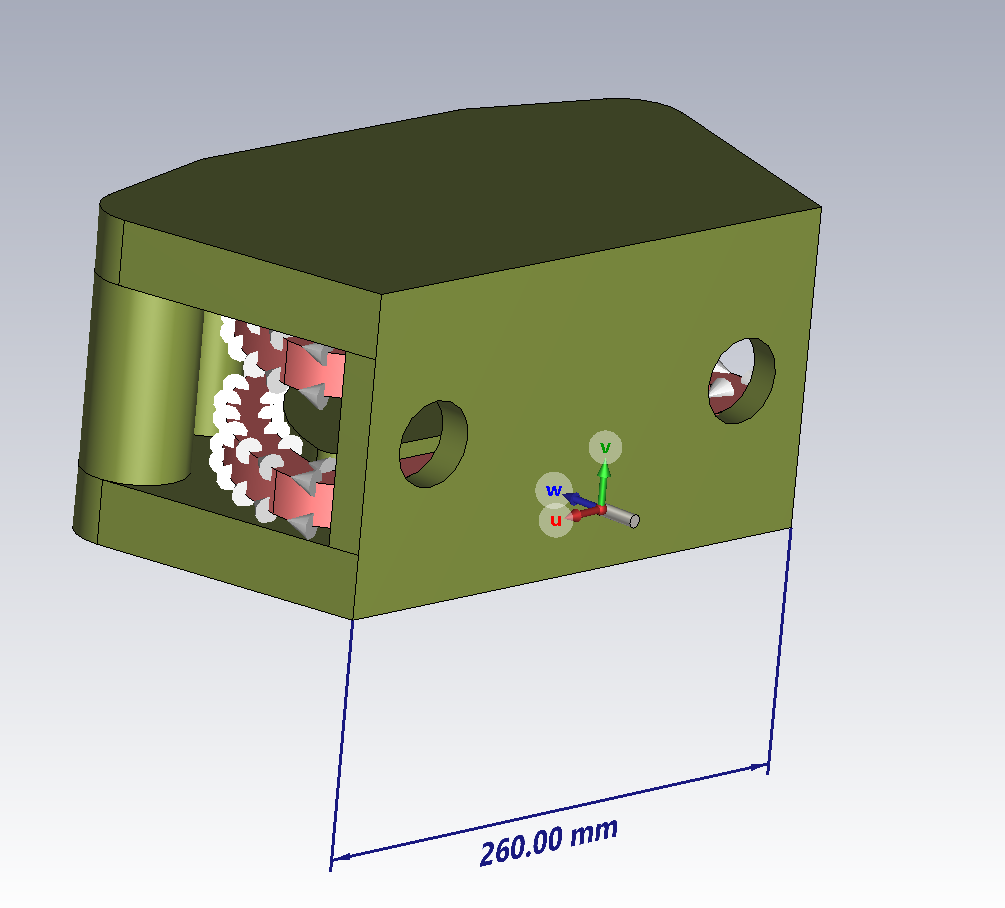
\includegraphics[width=.7\linewidth]{../../../figures/cst/cst_second_magnet_design1.png}
    \caption{Improved magnet design.}
    \label{fig:improved_magnet_design}
\end{figure}

\iffalse \begin{figure}[H]
    %\captionsetup[subfigure]{justification=centering}
    %\captionsetup{justification=centering}
    \centering
    \begin{subfigure}{.5\textwidth}
      \centering
      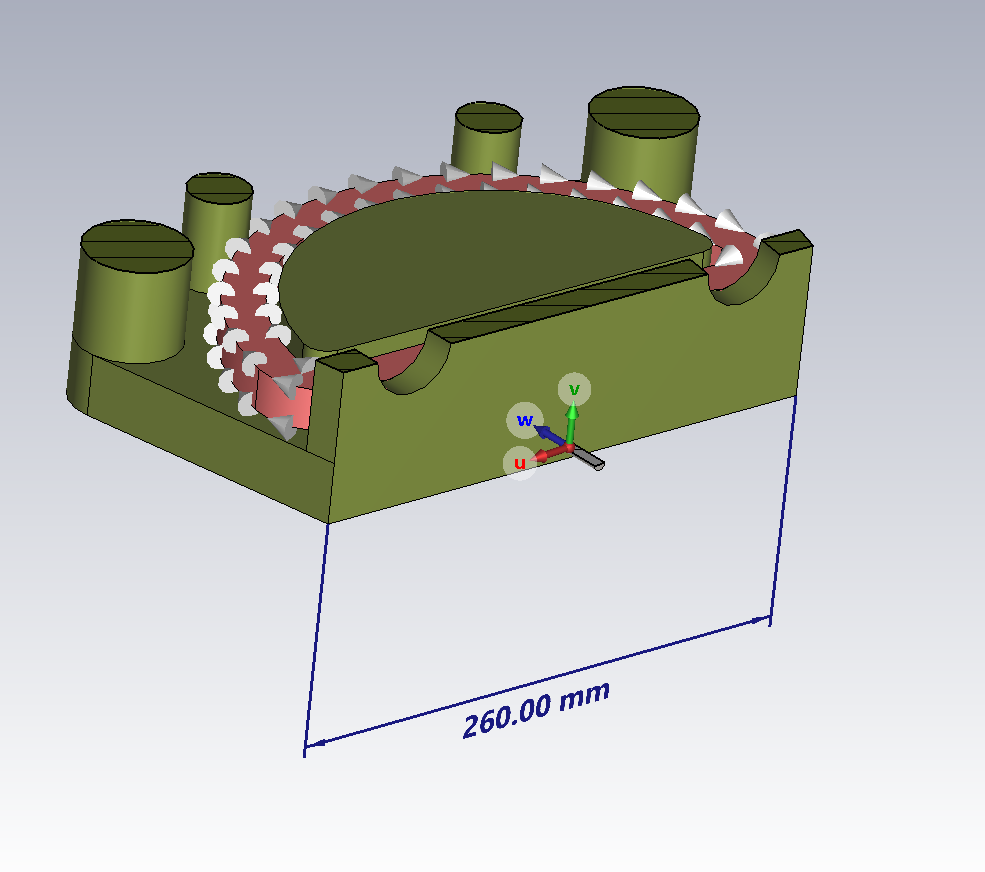
\includegraphics[width=.96\linewidth]{../../../figures/cst/cst_second_magnet_design2.png}
    \end{subfigure}%
    \centering
    \begin{subfigure}{.5\textwidth}
      \centering
      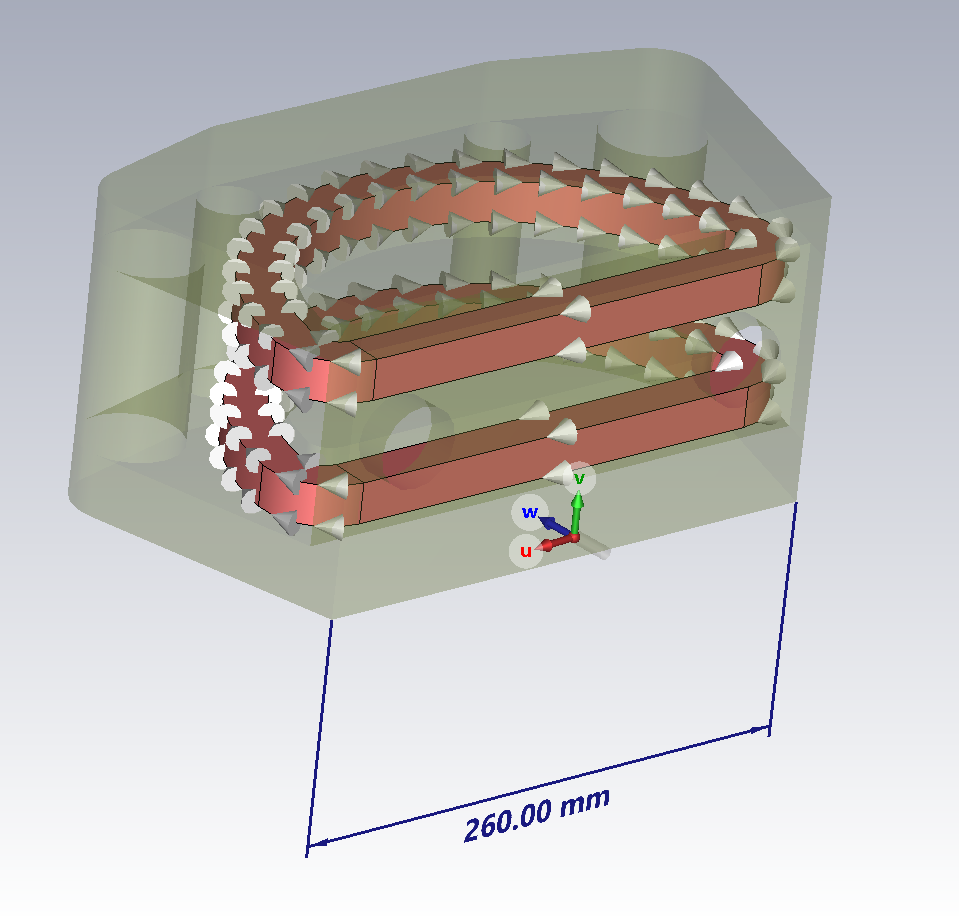
\includegraphics[width=.9\linewidth]{../../../figures/cst/cst_second_magnet_design3.png}
    \end{subfigure}
    \caption{Cross section and coils of improved magnet design.}
    \label{fig:improved_magnet_design_cross_section}
\end{figure} \fi
\begin{figure}[H]
    \centering
    \subfigure{{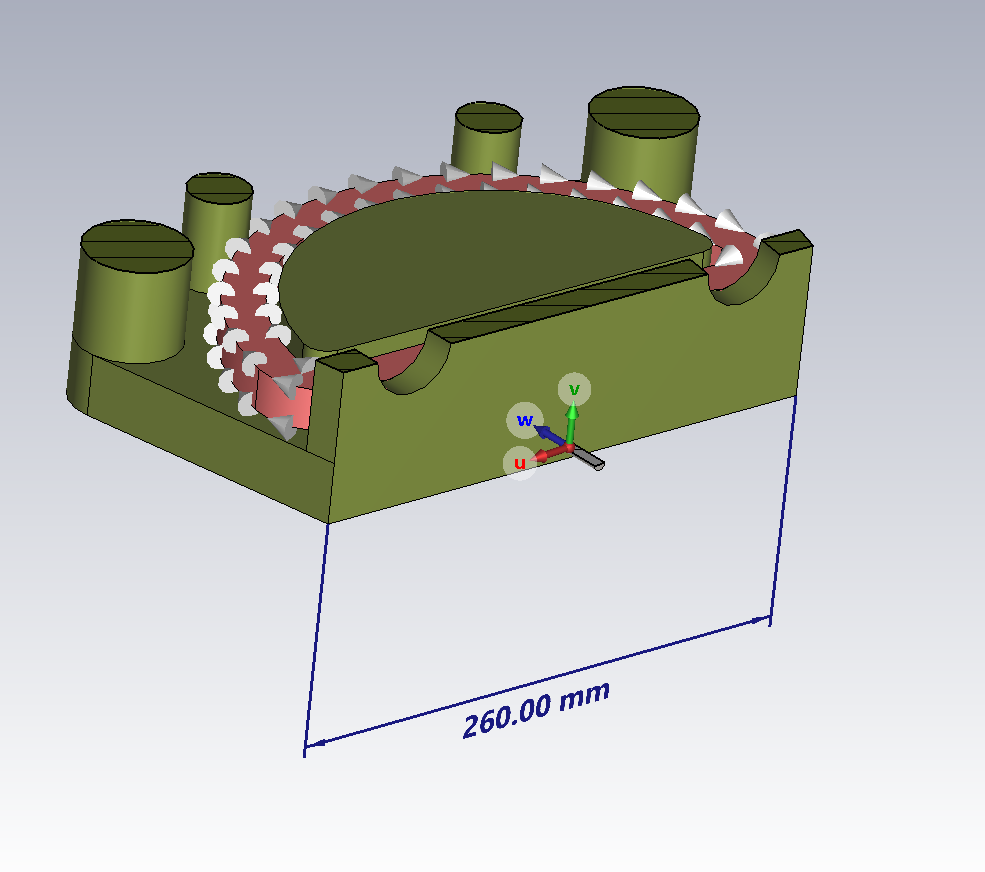
\includegraphics[width=.475\textwidth]{../../../figures/cst/cst_second_magnet_design2.png} }}%
    \qquad\subfigure{{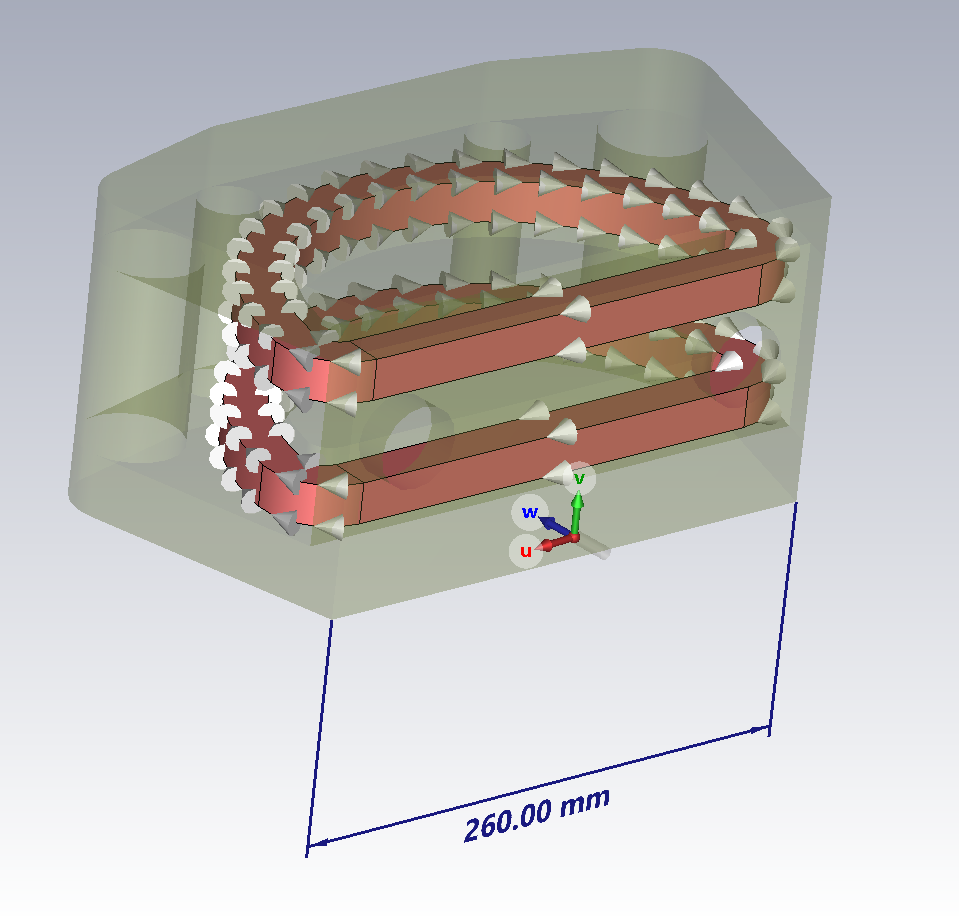
\includegraphics[width=.443\textwidth]{../../../figures/cst/cst_second_magnet_design3.png} }}%
    \vspace{20pt}
    \caption{\centering Cross section and coils of improved magnet design.} 
    \label{fig:improved_magnet_design_cross_section}
\end{figure}

\begin{figure}[H]
    \centering
    %%\captionsetup{justification=centering}
    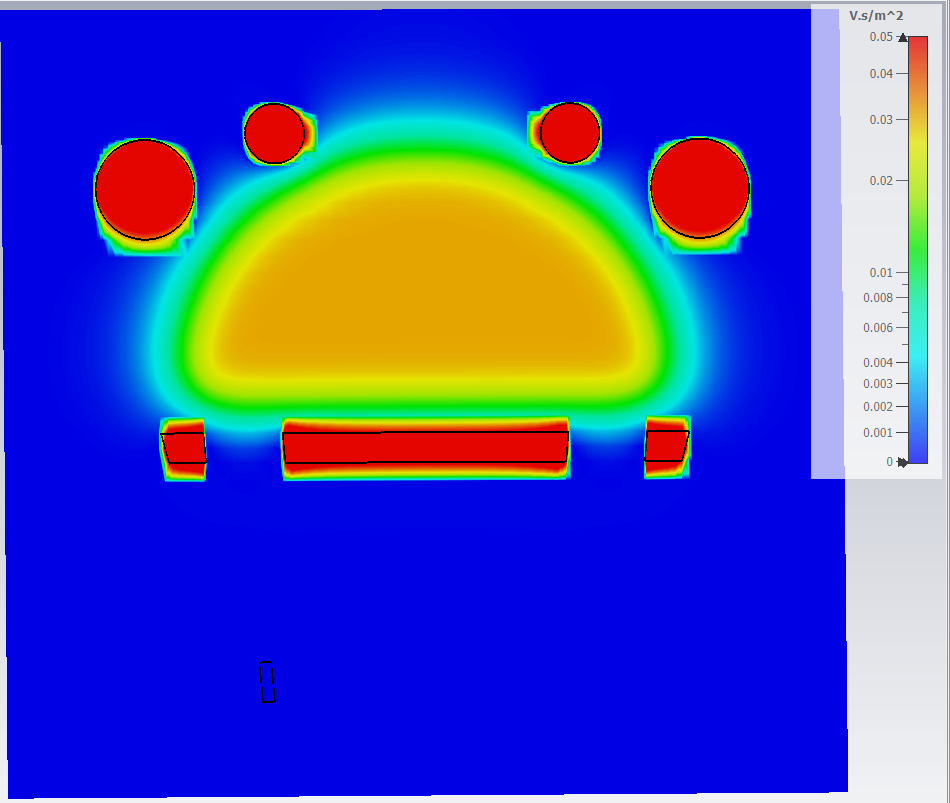
\includegraphics[width=.8\linewidth]{../../../figures/cst/cst_second_magnet_design4.png}
    \caption{Magnetic field in acceleration plate of improved magnet design.}
    \label{fig:improved_magnet_design_B}
\end{figure}
From \fromfigs{initial_magnet_design_B}{improved_magnet_design_B}, it can be observed that improved magnet design reduces magnetic field leak in enter and exit openings considerably. 
This reduction helps containing the spread of entering beam, decreasing the amount of focusing needed further into trajectory. 


%%%%%%


\end{document}